% !TeX spellcheck = de_DE
\section{Lunar Lander}
Die vorherigen Kapitel beschreiben die Ergebnisse des parallelisierten Verfahrens. Mit $40$ Prozessen wird ein \emph{SpeedUp} für die \emph{EvaluationTime} von $26.7$ und $29.6$ gemessen. Allerdings erfüllen die in diesen Umgebungen optimierten \ac{KNN} nicht die Eigenschaft der Generalisierung. Jedes \ac{KNN} beginnt die Evaluation immer in derselben Startposition und erzielt mit dieser gute Optimierungsergebnisse. Wenn diese \ac{KNN} in einer Umgebung mit einer abweichenden Startposition starten, besteht eine hohe Wahrscheinlichkeit, dass nicht das gewünschte Ergebnis erreicht wird. Bei der durchgeführten Analyse wird keine generelle Lösung für alle Startpositionen benötigt. Diese wäre zudem aufgrund der hohen Trainingszeiten ungeeignet. In diesem Kapitel wird ein letztes Optimierungsproblem aus dem OpenAI Gym mit dem Namen \emph{Lunar Lander} vorgestellt. Dieses Beispiel zeigt, wie eine generelle Lösung für alle Startsituation entwickelt werden kann und die hierfür benötigten Laufzeiten. 
Das Verfahren wird ausschließlich mit dem parallelisierten Algorithmus durchgeführt. Mit den zuvor gemessenen \emph{SpeedUp} Werten kann jedoch auf die Laufzeit des sequenziellen Verfahrens geschlossen werden.
\begin{figure}[!h]
	\centering
	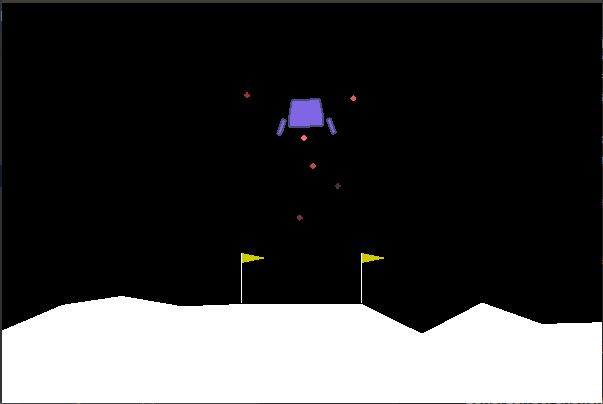
\includegraphics[width=0.5\textwidth]{./img/lunar_lander_env.JPG} 
	\caption{Darstellung der \emph{Lunar Lander} Umgebung aus dem OpenAI Gym}
	\label{fig:lunar_lander_env}
\end{figure} 
\\\\
Abbildung \ref{fig:lunar_lander_env} zeigt ein Raumschiff und eine Landeplattform, die sich zwischen zwei Fahnen befindet. Ziel der Umgebung ist das Landen des Raumschiffs auf der Plattform. Für das Optimierungsproblem stehen insgesamt $8$ Eingabewerte zur Verfügung, welche die Position, Geschwindigkeit und den Winkel des Raumschiffs beschreiben. Die Koordinaten der Landeplattform sind nicht enthalten, da sich diese immer an derselben Position befindet. Als Aktion kann entweder die sich unten am Raumschiff befindende Hauptdüse oder eine Steuerdüse an der linken oder rechten Seite des Raumschiffs aktiviert werden. Ebenfalls ist es möglich, den Antrieb nicht zu aktivieren und Treibstoff zu sparen. Die Simulation der Umgebung wird beendet, wenn das Raumschiff entweder abstürzt oder erfolgreich landet. Wie bei den anderen Umgebungen des OpenAI Gyms wird für jeden Zeitschritt ein \emph{reward} vergeben. Diese werden während der Simulation summiert und bilden den Fitnesswert. Ein positiver \emph{reward} wird vergeben, wenn das Raumschiff sinkt und sich der Plattform nähert. Zusätzlich gibt es einen Bonus, wenn das Raumschiff sich im Ziel befindet oder die Landefüße den Boden berühren. Für jeden Zeitschritt, in dem ein Antrieb aktiviert ist, wird ein kleiner Betrag vom \emph{reward} subtrahiert. Somit muss für die Maximierung des Fitnesswertes das Raumschiff so wenig Treibstoff wie möglich verbrauchen. Im Falle eines Absturzes gibt es einen negativen \emph{reward}.
\\\\
Für die Optimierung werden die Parameter der \emph{Pendulum} Umgebung übernommen. Somit steht eine Population von $1000$ Agenten zur Verfügung. Jedes \ac{KNN} besitzt entsprechend der Ein- und Ausgabewerte acht \emph{Input}- und vier \emph{Output}-Neuronen. Das Optimierungsproblem ist so konfiguriert, dass jeder Startzustand zufällig gewählt wird. Um eine generelle Lösungsstrategie zu finden, muss jeder Agent zehn Durchläufe in der Umgebung absolvieren. Für den finalen Fitnesswert werden die Ergebnisse der einzelnen Durchläufe summiert. Das Verfahren wird beendet, wenn ein Agent in jedem der zehn Durchläufe einen Fitnesswert von über $200$ Punkten erreicht. So ist sichergestellt, dass der Agent auf verschiedene Startsituationen entsprechend reagieren kann.
\begin{figure}[!h]
	\centering
	\begin{minipage}[]{0.49\textwidth}
		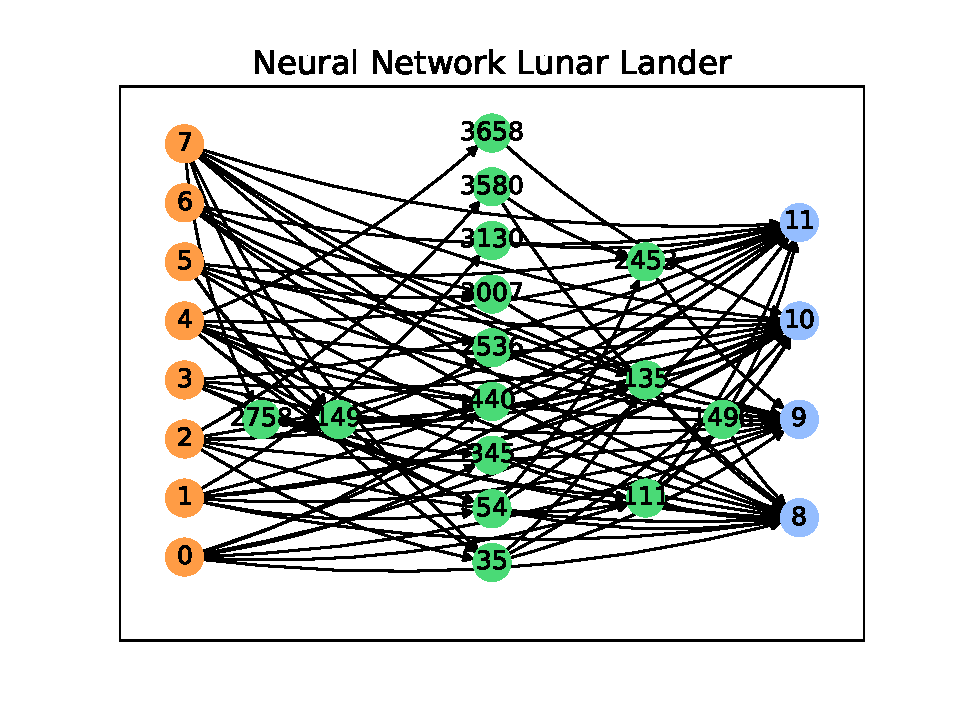
\includegraphics[width=1.0\textwidth]{./img/lunar_lander/lunar_lander_network.pdf} 
	\end{minipage}
	\hfill
	\begin{minipage}[]{0.49\textwidth}
		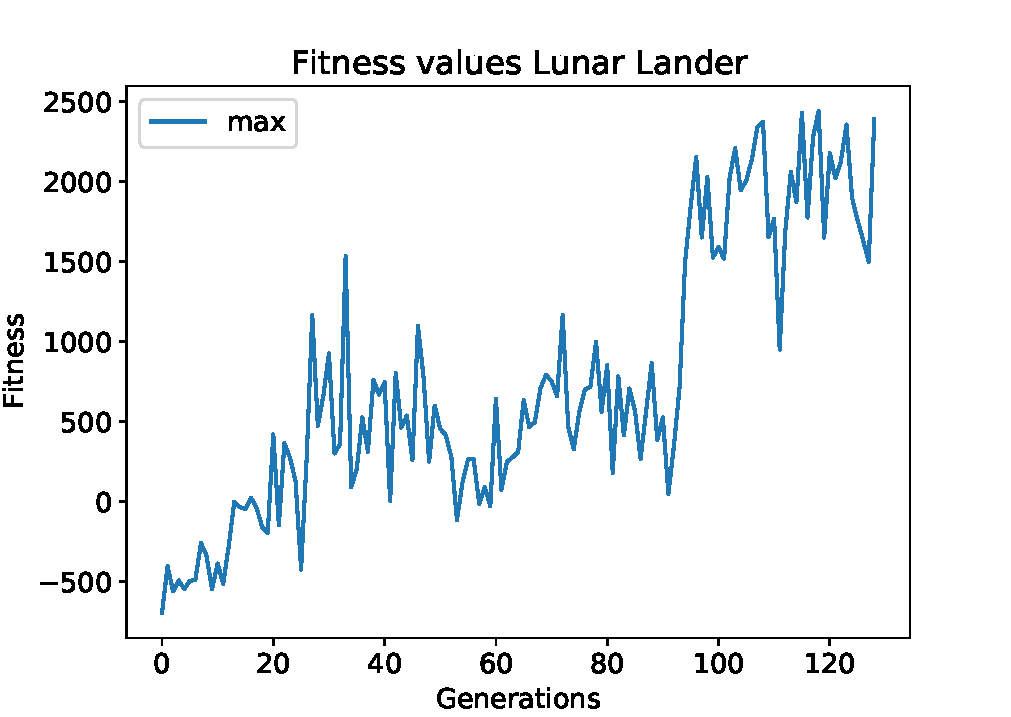
\includegraphics[width=1.0\textwidth]{./img/lunar_lander/lunar_lander_fitness.pdf} 
	\end{minipage}
	\caption{Links die Lösung für das \emph{Lunar Lander} Problem, rechts die dazugehörigen Fitnesswerte pro Generation}
	\label{fig:lunar_lander_neural_network_and_fitness}
\end{figure}
Abbildung \ref{fig:lunar_lander_neural_network_and_fitness} zeigt das finale \ac{KNN} und den Verlauf des maximalen Fitnesswertes. Das \ac{KNN} hat $15$ \emph{Hidden}-Neuronen entwickelt und besitzt insgesamt $88$ Verbindungen. Die Fitnesswerte sind anfänglich negativ, da das Raumschiff häufig abstürzt. Im weiteren Verlauf steigt der Fitnesswert zwar an, zeigt aber große Schwankungen aufgrund einer verrauschten Fitnessfunktion. Der Grund hierfür ist, dass nicht alle, sondern nur ein Teil der Startzustände evaluiert werden. So kann ein Agent hohe Fitnesswerte aufgrund günstiger Startpositionen erhalten, wie es zum Beispiel in Generation $33$ geschehen ist. In dieser hat der beste Agent einen Fitnesswert von $1533$ Punkten erzielt. Obwohl er unverändert in die nächste Generation kopiert wird, sinkt der maximale Fitnesswert auf $88$ Punkte. In Generation $94$ wird ein große Steigerung des Fitnesswertes auf $1495$ Punkte erzielt. Das Verfahren endet nach 128 Generationen mit einem Fitnesswert von $2394$ Punkten. Eine Besonderheit ist, dass der maximale Fitnesswert von $2441$ Punkten nicht am Ende des Verfahrens, sondern in Generation $118$ erzielt wird. 
Da jedoch die Abbruchbedingung nicht erfüllt ist, wird das Verfahren fortgeführt. Bei der Visualisierung des final entwickelten \ac{KNN} wird ersichtlich, dass das Verfahren grundsätzlich erfolgreich ist. Der Agent landet in vielen Fällen direkt auf der Zielplattform und erreicht Fitnesswerte zwischen $240$ bis $280$ Punkten. Allerdings gibt es auch Durchläufe, in denen der Agent abdriftet. In diesen Fällen landet das Raumschiff nicht auf der Plattform, dennoch werden Fitnesswerte von ungefähr $200$ Punkten erreicht. Insgesamt hat das Optimierungsverfahren eine generelle Lösungsstrategie entwickelt, aber die erreichten Fitnesswerte können aufgrund der unterschiedlichen Startpositionen dennoch abweichen. Eine bessere Leistung kann durch die Evaluation von weiteren Startzuständen oder eine höhere Trainingszeit erzielt werden.
\begin{figure}[!h]
	\centering
	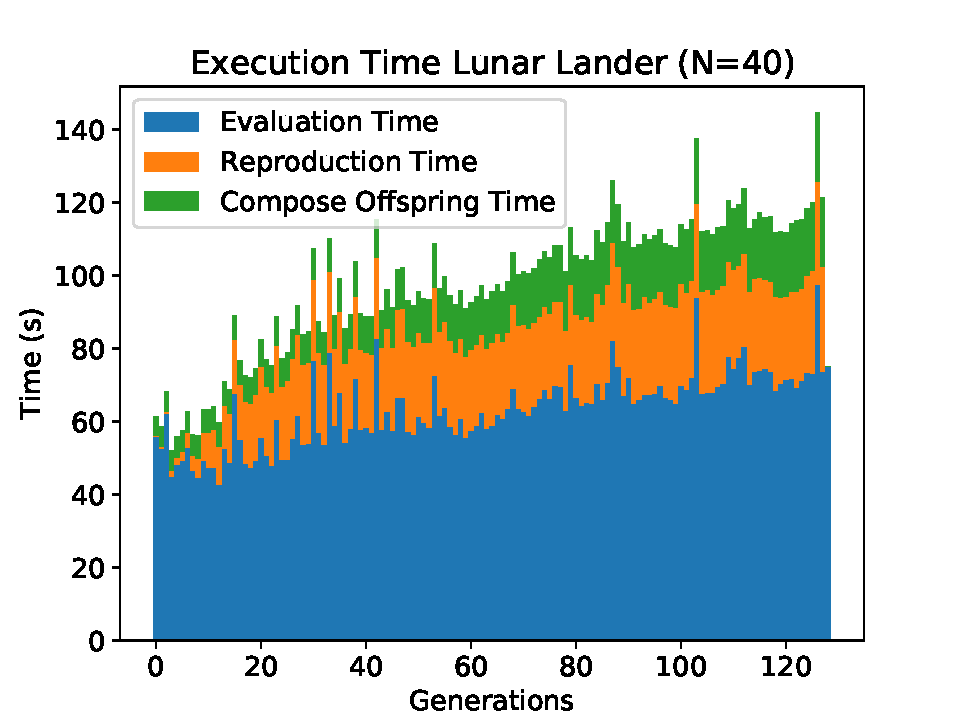
\includegraphics[width=0.7\textwidth]{./img/lunar_lander/lunar_lander_time_40.pdf} 
	\caption{Ausführungszeit des \emph{Lunar Lander} Problems auf 10 \emph{Raspberry Pis} mit 40 Prozessen}
	\label{fig:lunar_lander_time_40core_10pi}
\end{figure}
\\\\
Abbildung \ref{fig:lunar_lander_time_40core_10pi} zeigt die gemessenen Ausführungszeiten mit $40$ Prozessen auf zehn Raspberry Pis. Insgesamt hat das Verfahren etwa $3.5$ Stunden benötigt. Hiervon werden ungefähr $65\%$ für die \emph{Evaluation Time} verwendet. Der zweitgrößte Faktor der Ausführungszeit ist die \emph{Reproduction Time} mit ungefähr $22\%$, welcher wie bei der \emph{Pendulum} Umgebung durch die vielen verschiedenen Spezies zu erklären ist. Wie bei der \emph{Mountain Car} Umgebung unterliegt die Ausführungszeit der einzelnen Generationen einigen Schwankungen, da die Evaluationszeit je nach Agent stark abweichen kann. Stürzt das Raumschiff direkt ab oder landet schnell, ist die Evaluationszeit kurz. Evaluationen mit einer hohen Flugzeit können hingegen vergleichsweise lange andauern. Auch die Größe des \ac{KNN} kann ein entscheidender Faktor sein, sowohl bei der \emph{Evaluation} als auch in den Phasen \emph{Mutation} und \emph{Rekombination}. Um in solchen Szenarien gute Effizienzwerte zu erhalten, ist die dynamische Zuteilung von Arbeitspaketen durch die \emph{Master-Slave} Architektur besonders wichtig. Prinzipiell hätte diese Umgebung auch bei der Analyse in Kapitel \ref{chap:analysis} verwendet werden können, die lange Ausführungszeit ist jedoch nicht praktikabel. Mit den \emph{SpeedUp} Werten aus der \emph{Mountain Car} und \emph{Pendulum} Umgebung ist auf die sequenzielle Ausführungszeit zu schließen. Bei einem \emph{SpeedUp} Faktor von $26.7$ bzw. $29.6$ liegt die erwartete Ausführungszeit zwischen $62.1$ und $68.7$ Stunden. 